% Options for packages loaded elsewhere
\PassOptionsToPackage{unicode}{hyperref}
\PassOptionsToPackage{hyphens}{url}
\PassOptionsToPackage{dvipsnames,svgnames,x11names}{xcolor}
%
\documentclass[
  letterpaper,
  DIV=11,
  numbers=noendperiod]{scrartcl}

\usepackage{amsmath,amssymb}
\usepackage{iftex}
\ifPDFTeX
  \usepackage[T1]{fontenc}
  \usepackage[utf8]{inputenc}
  \usepackage{textcomp} % provide euro and other symbols
\else % if luatex or xetex
  \usepackage{unicode-math}
  \defaultfontfeatures{Scale=MatchLowercase}
  \defaultfontfeatures[\rmfamily]{Ligatures=TeX,Scale=1}
\fi
\usepackage{lmodern}
\ifPDFTeX\else  
    % xetex/luatex font selection
\fi
% Use upquote if available, for straight quotes in verbatim environments
\IfFileExists{upquote.sty}{\usepackage{upquote}}{}
\IfFileExists{microtype.sty}{% use microtype if available
  \usepackage[]{microtype}
  \UseMicrotypeSet[protrusion]{basicmath} % disable protrusion for tt fonts
}{}
\makeatletter
\@ifundefined{KOMAClassName}{% if non-KOMA class
  \IfFileExists{parskip.sty}{%
    \usepackage{parskip}
  }{% else
    \setlength{\parindent}{0pt}
    \setlength{\parskip}{6pt plus 2pt minus 1pt}}
}{% if KOMA class
  \KOMAoptions{parskip=half}}
\makeatother
\usepackage{xcolor}
\setlength{\emergencystretch}{3em} % prevent overfull lines
\setcounter{secnumdepth}{-\maxdimen} % remove section numbering
% Make \paragraph and \subparagraph free-standing
\ifx\paragraph\undefined\else
  \let\oldparagraph\paragraph
  \renewcommand{\paragraph}[1]{\oldparagraph{#1}\mbox{}}
\fi
\ifx\subparagraph\undefined\else
  \let\oldsubparagraph\subparagraph
  \renewcommand{\subparagraph}[1]{\oldsubparagraph{#1}\mbox{}}
\fi

\usepackage{color}
\usepackage{fancyvrb}
\newcommand{\VerbBar}{|}
\newcommand{\VERB}{\Verb[commandchars=\\\{\}]}
\DefineVerbatimEnvironment{Highlighting}{Verbatim}{commandchars=\\\{\}}
% Add ',fontsize=\small' for more characters per line
\usepackage{framed}
\definecolor{shadecolor}{RGB}{241,243,245}
\newenvironment{Shaded}{\begin{snugshade}}{\end{snugshade}}
\newcommand{\AlertTok}[1]{\textcolor[rgb]{0.68,0.00,0.00}{#1}}
\newcommand{\AnnotationTok}[1]{\textcolor[rgb]{0.37,0.37,0.37}{#1}}
\newcommand{\AttributeTok}[1]{\textcolor[rgb]{0.40,0.45,0.13}{#1}}
\newcommand{\BaseNTok}[1]{\textcolor[rgb]{0.68,0.00,0.00}{#1}}
\newcommand{\BuiltInTok}[1]{\textcolor[rgb]{0.00,0.23,0.31}{#1}}
\newcommand{\CharTok}[1]{\textcolor[rgb]{0.13,0.47,0.30}{#1}}
\newcommand{\CommentTok}[1]{\textcolor[rgb]{0.37,0.37,0.37}{#1}}
\newcommand{\CommentVarTok}[1]{\textcolor[rgb]{0.37,0.37,0.37}{\textit{#1}}}
\newcommand{\ConstantTok}[1]{\textcolor[rgb]{0.56,0.35,0.01}{#1}}
\newcommand{\ControlFlowTok}[1]{\textcolor[rgb]{0.00,0.23,0.31}{#1}}
\newcommand{\DataTypeTok}[1]{\textcolor[rgb]{0.68,0.00,0.00}{#1}}
\newcommand{\DecValTok}[1]{\textcolor[rgb]{0.68,0.00,0.00}{#1}}
\newcommand{\DocumentationTok}[1]{\textcolor[rgb]{0.37,0.37,0.37}{\textit{#1}}}
\newcommand{\ErrorTok}[1]{\textcolor[rgb]{0.68,0.00,0.00}{#1}}
\newcommand{\ExtensionTok}[1]{\textcolor[rgb]{0.00,0.23,0.31}{#1}}
\newcommand{\FloatTok}[1]{\textcolor[rgb]{0.68,0.00,0.00}{#1}}
\newcommand{\FunctionTok}[1]{\textcolor[rgb]{0.28,0.35,0.67}{#1}}
\newcommand{\ImportTok}[1]{\textcolor[rgb]{0.00,0.46,0.62}{#1}}
\newcommand{\InformationTok}[1]{\textcolor[rgb]{0.37,0.37,0.37}{#1}}
\newcommand{\KeywordTok}[1]{\textcolor[rgb]{0.00,0.23,0.31}{#1}}
\newcommand{\NormalTok}[1]{\textcolor[rgb]{0.00,0.23,0.31}{#1}}
\newcommand{\OperatorTok}[1]{\textcolor[rgb]{0.37,0.37,0.37}{#1}}
\newcommand{\OtherTok}[1]{\textcolor[rgb]{0.00,0.23,0.31}{#1}}
\newcommand{\PreprocessorTok}[1]{\textcolor[rgb]{0.68,0.00,0.00}{#1}}
\newcommand{\RegionMarkerTok}[1]{\textcolor[rgb]{0.00,0.23,0.31}{#1}}
\newcommand{\SpecialCharTok}[1]{\textcolor[rgb]{0.37,0.37,0.37}{#1}}
\newcommand{\SpecialStringTok}[1]{\textcolor[rgb]{0.13,0.47,0.30}{#1}}
\newcommand{\StringTok}[1]{\textcolor[rgb]{0.13,0.47,0.30}{#1}}
\newcommand{\VariableTok}[1]{\textcolor[rgb]{0.07,0.07,0.07}{#1}}
\newcommand{\VerbatimStringTok}[1]{\textcolor[rgb]{0.13,0.47,0.30}{#1}}
\newcommand{\WarningTok}[1]{\textcolor[rgb]{0.37,0.37,0.37}{\textit{#1}}}

\providecommand{\tightlist}{%
  \setlength{\itemsep}{0pt}\setlength{\parskip}{0pt}}\usepackage{longtable,booktabs,array}
\usepackage{calc} % for calculating minipage widths
% Correct order of tables after \paragraph or \subparagraph
\usepackage{etoolbox}
\makeatletter
\patchcmd\longtable{\par}{\if@noskipsec\mbox{}\fi\par}{}{}
\makeatother
% Allow footnotes in longtable head/foot
\IfFileExists{footnotehyper.sty}{\usepackage{footnotehyper}}{\usepackage{footnote}}
\makesavenoteenv{longtable}
\usepackage{graphicx}
\makeatletter
\def\maxwidth{\ifdim\Gin@nat@width>\linewidth\linewidth\else\Gin@nat@width\fi}
\def\maxheight{\ifdim\Gin@nat@height>\textheight\textheight\else\Gin@nat@height\fi}
\makeatother
% Scale images if necessary, so that they will not overflow the page
% margins by default, and it is still possible to overwrite the defaults
% using explicit options in \includegraphics[width, height, ...]{}
\setkeys{Gin}{width=\maxwidth,height=\maxheight,keepaspectratio}
% Set default figure placement to htbp
\makeatletter
\def\fps@figure{htbp}
\makeatother

\usepackage{booktabs}
\usepackage{longtable}
\usepackage{array}
\usepackage{multirow}
\usepackage{wrapfig}
\usepackage{float}
\usepackage{colortbl}
\usepackage{pdflscape}
\usepackage{tabu}
\usepackage{threeparttable}
\usepackage{threeparttablex}
\usepackage[normalem]{ulem}
\usepackage{makecell}
\usepackage{xcolor}
\usepackage[auth-lg]{authblk}
\KOMAoption{captions}{tableheading}
\makeatletter
\makeatother
\makeatletter
\makeatother
\makeatletter
\@ifpackageloaded{caption}{}{\usepackage{caption}}
\AtBeginDocument{%
\ifdefined\contentsname
  \renewcommand*\contentsname{Table of contents}
\else
  \newcommand\contentsname{Table of contents}
\fi
\ifdefined\listfigurename
  \renewcommand*\listfigurename{List of Figures}
\else
  \newcommand\listfigurename{List of Figures}
\fi
\ifdefined\listtablename
  \renewcommand*\listtablename{List of Tables}
\else
  \newcommand\listtablename{List of Tables}
\fi
\ifdefined\figurename
  \renewcommand*\figurename{Figure}
\else
  \newcommand\figurename{Figure}
\fi
\ifdefined\tablename
  \renewcommand*\tablename{Table}
\else
  \newcommand\tablename{Table}
\fi
}
\@ifpackageloaded{float}{}{\usepackage{float}}
\floatstyle{ruled}
\@ifundefined{c@chapter}{\newfloat{codelisting}{h}{lop}}{\newfloat{codelisting}{h}{lop}[chapter]}
\floatname{codelisting}{Listing}
\newcommand*\listoflistings{\listof{codelisting}{List of Listings}}
\makeatother
\makeatletter
\@ifpackageloaded{caption}{}{\usepackage{caption}}
\@ifpackageloaded{subcaption}{}{\usepackage{subcaption}}
\makeatother
\makeatletter
\@ifpackageloaded{tcolorbox}{}{\usepackage[skins,breakable]{tcolorbox}}
\makeatother
\makeatletter
\@ifundefined{shadecolor}{\definecolor{shadecolor}{rgb}{.97, .97, .97}}
\makeatother
\makeatletter
\makeatother
\makeatletter
\makeatother
\ifLuaTeX
  \usepackage{selnolig}  % disable illegal ligatures
\fi
\IfFileExists{bookmark.sty}{\usepackage{bookmark}}{\usepackage{hyperref}}
\IfFileExists{xurl.sty}{\usepackage{xurl}}{} % add URL line breaks if available
\urlstyle{same} % disable monospaced font for URLs
\hypersetup{
  pdftitle={Trabalho Prático 1},
  pdfauthor={Ana Theresa Figueiredo - 18/0116088; César Augusto Galvão - 19/0011572},
  colorlinks=true,
  linkcolor={blue},
  filecolor={Maroon},
  citecolor={Blue},
  urlcolor={Blue},
  pdfcreator={LaTeX via pandoc}}

\title{Trabalho Prático 1}
\usepackage{etoolbox}
\makeatletter
\providecommand{\subtitle}[1]{% add subtitle to \maketitle
  \apptocmd{\@title}{\par {\large #1 \par}}{}{}
}
\makeatother
\subtitle{Análise de Séries Temporais - 1/2023}
\author{Ana Theresa Figueiredo - 18/0116088 \and César Augusto Galvão -
19/0011572}
\date{}

\begin{document}
\maketitle
\ifdefined\Shaded\renewenvironment{Shaded}{\begin{tcolorbox}[enhanced, boxrule=0pt, interior hidden, breakable, sharp corners, borderline west={3pt}{0pt}{shadecolor}, frame hidden]}{\end{tcolorbox}}\fi

\renewcommand*\contentsname{Table of contents}
{
\hypersetup{linkcolor=}
\setcounter{tocdepth}{3}
\tableofcontents
}
\newpage{}

\hypertarget{introduuxe7uxe3o}{%
\section{Introdução}\label{introduuxe7uxe3o}}

A série temporal escolhida foi a de número \emph{id} correspondente a
2546. De acordo com a definição do próprio pacote, refere-se a
\emph{Large commercial banks, commercial \& industrial loans}, ou seja,
dados financeiros e de impréstimos industriais e comerciais. Foram
realizadas medidas mensais de 1983 a 1992 e o horizonte de previsão
requerido é das 18 ocorrências seguintes.

O gráfico da série, com \emph{in} e \emph{out-sample}, é exposto a
seguir.

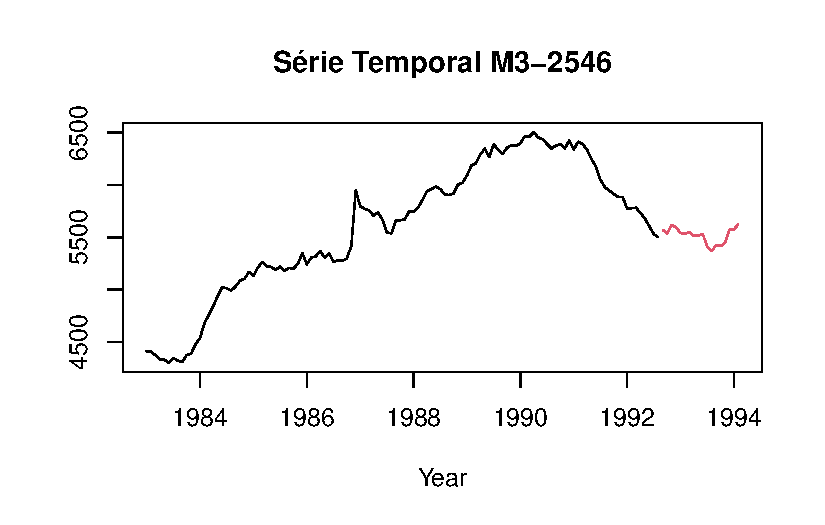
\includegraphics{T1_grupo15_files/figure-pdf/plot-serie-total-1.pdf}

\hypertarget{a.-decomposiuxe7uxe3o-da-suxe9rie-temporal.}{%
\section{a. Decomposição da série
temporal.}\label{a.-decomposiuxe7uxe3o-da-suxe9rie-temporal.}}

Inicia-se a decomposição utilizando STL, caso em que se utiliza uma
decomposição Loess. O gráfico dos resultados da função \texttt{stl()}
são expostos a seguir utilizando os argumentos \texttt{s.window} e
\texttt{t.window} iguais a sete. Esta configuração de argumentos foi
escolhida após algumas iterações -- balizada também por recomendações de
Cleveland \emph{et al.} (1990) -- buscando, entre outros fatores, um
comportamento adequado dos resíduos do modelo.

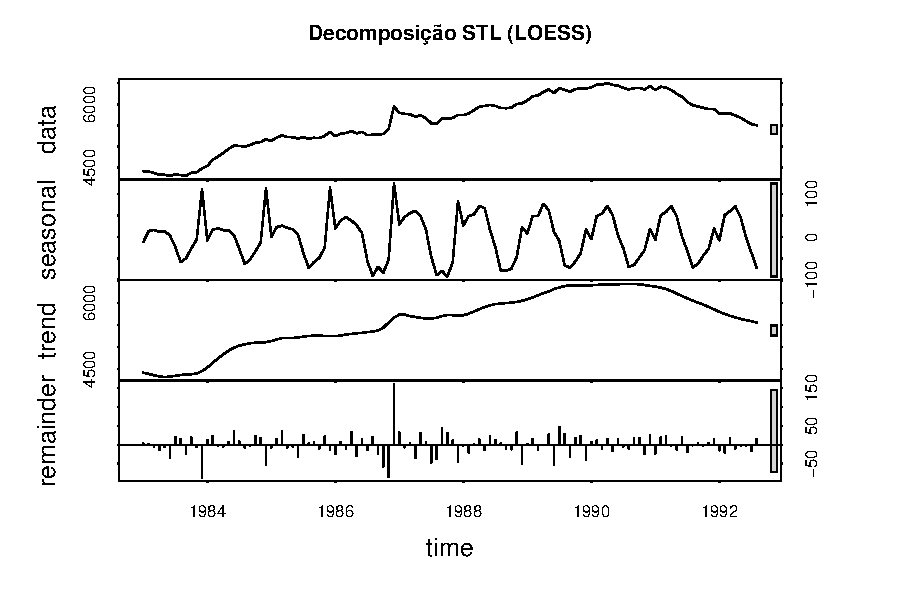
\includegraphics{T1_grupo15_files/figure-pdf/STL-1.pdf}

De fato, observa-se uma tendência crescente até 1990, além de parecer
haver também uma sazonalidade anual. Esta apresenta alguns picos mais
intensos no começo dos ciclos periódicos e menos intensos na segunda
metade da série.

Além disso, o termo aleatório parece estável a menos de um pico em 1987,
característica que orientou a escolha dos valores para \texttt{t.window}
e \texttt{s.window}. Esses argumentos (\ldots)

\textbf{DESCREVER O QUE T.WINDOW E S.WINDOW FAZEM}

Experimenta-se também a decomposição via MSTL, procurando uma
sazonalidade múltipla, sugerida pelos picos nos inícios das ondas
sazonais. Após algumas iterações, optou-se pelo período bimestral,
complementarmente ao período mensal original da série. Os mesmos valores
para os argumentos de janela foram utilizados.

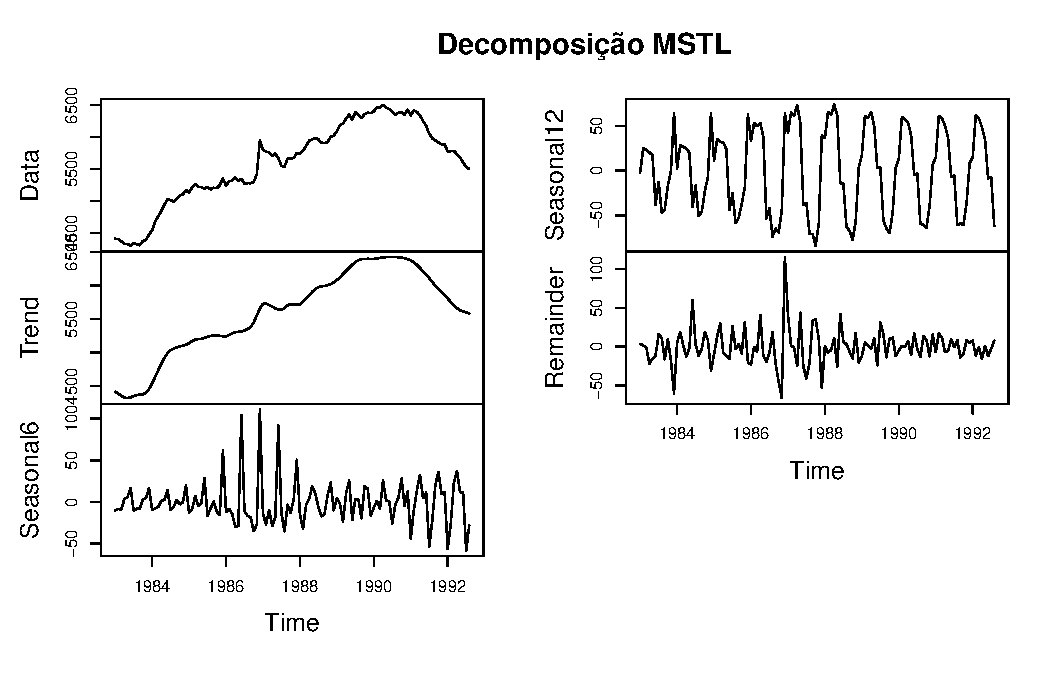
\includegraphics{T1_grupo15_files/figure-pdf/unnamed-chunk-1-1.pdf}

De fato, conseguiu-se remover o pico inicial da sazonalidade simples. No
entanto, nota-se uma variação grande nas amplitudes sazonais, assim como
homocedasticidade do resíduo.

Opta-se finalmente pela decomposição STL, com sazonalidade simples.

\hypertarget{b.-escolha-um-modelo-arima}{%
\section{b. Escolha um modelo ARIMA}\label{b.-escolha-um-modelo-arima}}

\begin{itemize}
\tightlist
\item
  O modelo selecionado deve ser baseado no que você visualizou na
  decomposição, testes estatísticos, gráficos ACF, gráficos PACF,
  critérios de parcimonia e resíduos;
\item
  Detalhe todo o procedimento da escolha do modelo;
\item
  Nao pode usar AutoArima
\item
  Tem q fazer o algorito mostrado em sala.
\end{itemize}

Para selecionar o modelo ARIMA, iniciamos pela identificação das
diferenciações sazonais e não sazonais utilizando as funções
\texttt{nsdiffs()} e \texttt{ndiffs()}, respectivamente, do pacote
\texttt{forecast}. Dessa forma, para um modelo
\(\text{SARIMA}(p,d,q)\times(P,D,Q)_{12}\) ou
\(\text{SARMA}(P,Q)_{12}\), obtemos os valores de \(D\) e \(d\).

Isto feito, sabemos que o modelo é pelo menos
\((p,2,q)\times(P,0,Q)_{12}\).

\hypertarget{estacionariedade-da-suxe9rie}{%
\subsection{Estacionariedade da
série}\label{estacionariedade-da-suxe9rie}}

Antes de prosseguir, avalia-se a estacionariedade da série. Para isso,
utiliza-se o teste KPSS (Kwiatkowski \emph{et al.}, 1992. As hipóteses
do teste são:

\[
\begin{aligned}
  &H_0: \text{o processo é estacionário} \\
  &H_1: \text{o processo possui raiz unitária}
\end{aligned}
\] Os resultados do teste são exibidos na tabela a seguir, sugerindo não
rejeitar a hipótese de estacionariedade.

\begin{longtable*}{ccc}
\toprule
Estatística de teste & p-valor & Método\\
\midrule
\endfirsthead
\multicolumn{3}{@{}l}{\textit{(continued)}}\\
\toprule
Estatística de teste & p-valor & Método\\
\midrule
\endhead

\endfoot
\bottomrule
\endlastfoot
\cellcolor{gray!15}{0.0244372} & \cellcolor{gray!15}{0.1} & \cellcolor{gray!15}{KPSS Test for Level Stationarity}\\*
\end{longtable*}

\hypertarget{anuxe1lise-gruxe1fica-fac-e-facp}{%
\section{Análise gráfica FAC e
FACP}\label{anuxe1lise-gruxe1fica-fac-e-facp}}

A seguir são expostos três gráficos para a série diferenciada em
\(\nabla^2x_t\): a série original com duas diferenciações simples
(portanto estacionária), sua Função de Autocorrelação - FAC (\emph{ACF})
e a Função de Autocorrelação Parcial - FACP (\emph{Partial ACF}).

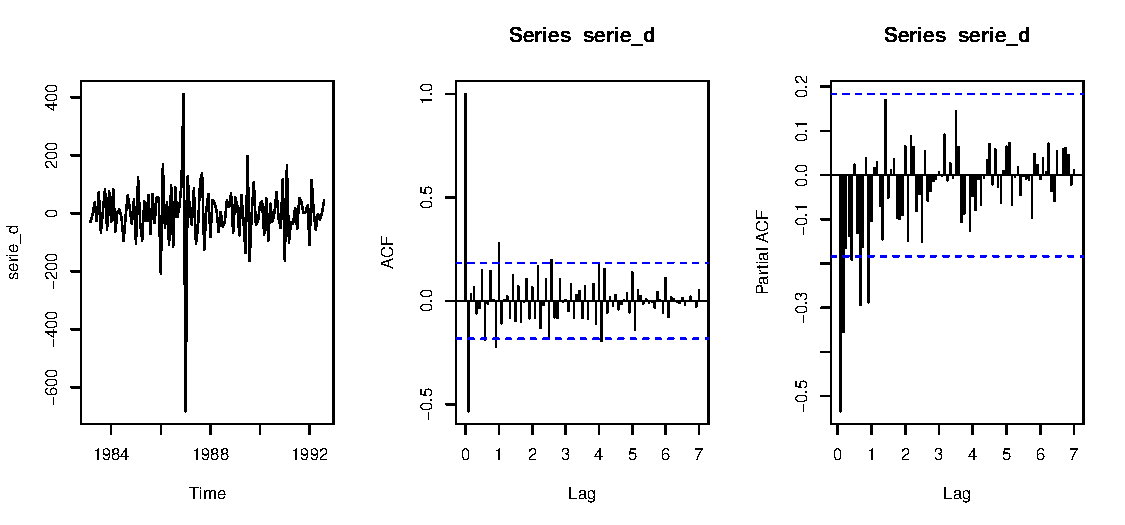
\includegraphics{T1_grupo15_files/figure-pdf/FAC-FACP-1.pdf}

Nota-se um decaimento amortecido no gráfico FAC e poucas correlações
fora da banda apenas até Lag 1 do FACP. As autocorrelações parciais, no
entanto, também decaem de forma amortecida para zero sem quebras. Este
comportamento indica candidatos a modelos ARIMA ou SARMA.

\hypertarget{anuxe1lise-iterativa}{%
\subsection{Análise iterativa}\label{anuxe1lise-iterativa}}

Na falta de comportamentos claros indicando os demais coeficientes,
recorre-se a uma varredura para selecionar o modelo mais parcimonioso
utilizando AICc como critério.

Conforme a saída a seguir, verifica-se uma boa configuração sendo
\(\text{SARMA}(0,2,1)\times(1,0,0)\)

\begin{verbatim}
[1] "p = 0, q = 1, P = 1, Q = 0, AICc = 1313.1422"
[2] "p = 0, q = 1, P = 0, Q = 1, AICc = 1313.8014"
[3] "p = 0, q = 1, P = 0, Q = 0, AICc = 1318.3233"
[4] "p = 0, q = 0, P = 1, Q = 0, AICc = 1380.2924"
[5] "p = 0, q = 0, P = 0, Q = 1, AICc = 1380.984" 
[6] "p = 0, q = 0, P = 0, Q = 0, AICc = 1387.0622"
\end{verbatim}

Finalmente, ajusta-se o modelo conforme as especificações e obtém-se os
seguintes coeficientes:

\begin{longtable*}{cc}
\toprule
Coeficiente & Valor\\
\midrule
\endfirsthead
\multicolumn{2}{@{}l}{\textit{(continued)}}\\
\toprule
Coeficiente & Valor\\
\midrule
\endhead

\endfoot
\bottomrule
\endlastfoot
\cellcolor{gray!15}{ma1} & \cellcolor{gray!15}{-0.8394}\\
sar1 & 0.2545\\*
\end{longtable*}

\hypertarget{c.-anuxe1lise-de-resuxedduos-do-modelo-selecionado.}{%
\section{c.~Análise de resíduos do modelo
selecionado.}\label{c.-anuxe1lise-de-resuxedduos-do-modelo-selecionado.}}

Para avaliar a qualidade do modelo, verifica-se as seguintes suposições
sobre \(\{\varepsilon_t\}\):

\begin{itemize}
\tightlist
\item
  Média zero,
\item
  Variância constante,
\item
  Autocorrelação nula,
\item
  Normalidade.
\end{itemize}

Verifica-se inicialmente a série dos resíduos sem a incialização com
zeros. Graficamente, pode-se dizer que tem média igual a zero. De fato,
a média calculada dos resíduos corresponde a -9.495, o que é muito
próximo de zero considerando a ordem de grandeza de muitos valores dos
resíduos. Além disso, a variância parece ser constante, a menos do pico
no meio da série.

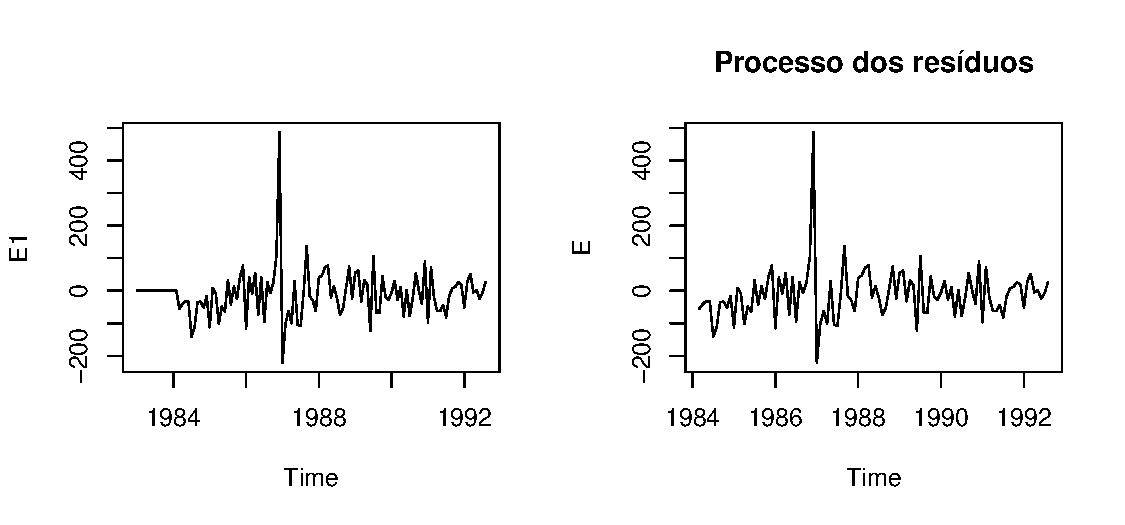
\includegraphics{T1_grupo15_files/figure-pdf/dist-residuos-1.pdf}

O Q-Q Plot a seguir aponta uma proximidade não ideal em relação à
distribuição normal com uma caudal mais pesada à esquerda e um ponto
extremo à direita. Além disso, o ACF possui uma quebra na banda de
confiança, mas mantém as demais autocorrelações dentro dos limites.

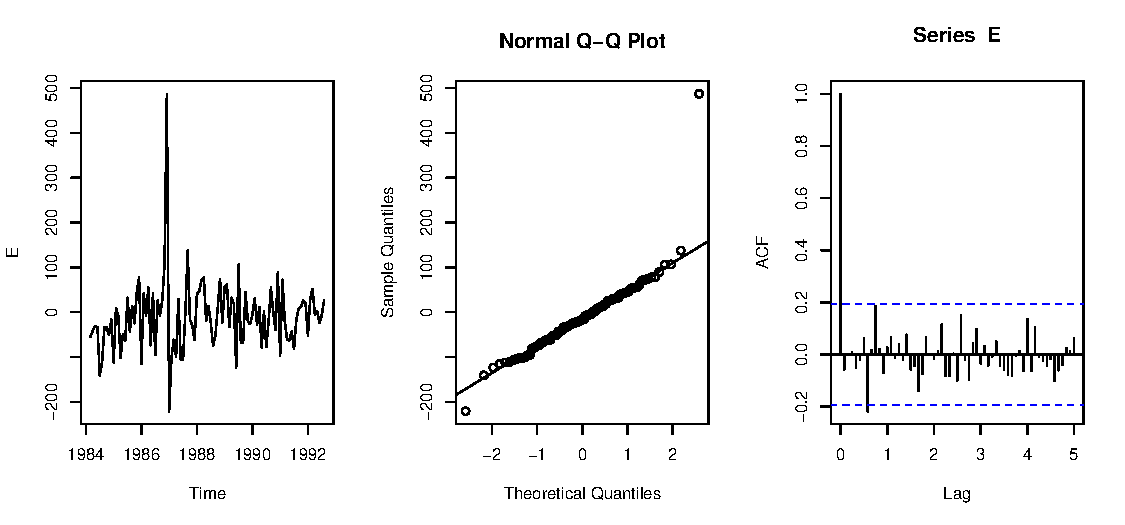
\includegraphics{T1_grupo15_files/figure-pdf/unnamed-chunk-3-1.pdf}

Por fim, verifica-se utilizando testes de hipótese estacionariedade
(\(H_0:\) o processo é estacionário), independência
(\(H_0: \rho(1) = \rho(2), = \dots = \rho(m) = 0\)) e normalidade
(\(H_0:\) não se rejeita normalidade) dos resíduos do modelo.

Infere-se pelos testes que se trata de uma série estacionária, com
autocorrelações todas iguais a zero, porém não normal. Isso
provavelmente ocorre por causa de um peso maior na cauda esquerda e por
causa da presença de alguns valores extremos.

\begin{longtable*}{ccc}
\toprule
Estatística de teste & p-valor & Método\\
\midrule
\endfirsthead
\multicolumn{3}{@{}l}{\textit{(continued)}}\\
\toprule
Estatística de teste & p-valor & Método\\
\midrule
\endhead

\endfoot
\bottomrule
\endlastfoot
\cellcolor{gray!15}{0.2061} & \cellcolor{gray!15}{0.1000} & \cellcolor{gray!15}{KPSS Test for Level Stationarity}\\
15.7901 & 0.7296 & Box-Ljung test\\
\cellcolor{gray!15}{0.8363} & \cellcolor{gray!15}{0.0000} & \cellcolor{gray!15}{Shapiro-Wilk normality test}\\*
\end{longtable*}

\hypertarget{d.-apresentauxe7uxe3o-do-modelo-selecionado}{%
\section{d.~Apresentação do modelo
selecionado}\label{d.-apresentauxe7uxe3o-do-modelo-selecionado}}

O modelo selecionado é, conforme ja apresentado,
\(\text{SARMA}(0,2,1)\times(1,0,0)_{12}\). Em forma polinomial temos:

\[
\begin{aligned}
  \Phi_P(B^s)x_t =& \, \Theta(B)\varepsilon_t \\
  \Phi_1(B)x_t =& \, \Theta_1(B)\varepsilon_t\\
  (1-\phi_1 B)x_t =& \, (1+\theta_1 B)\varepsilon_t \\
  x_t - \phi_1 x_{t-1} =& \, \varepsilon_t  + \theta_1 \varepsilon_{t-1} \\
  x_t  =& \, \varepsilon_t  + \theta_1 \varepsilon_{t-1} + \phi_1 x_{t-1}\\
  x_t  =& \, \varepsilon_t  -0.839 \, \varepsilon_{t-1} + 0.255 \, x_{t-1}
\end{aligned}
\]

\hypertarget{comparauxe7uxe3o-auto.arima}{%
\section{Comparação auto.arima()}\label{comparauxe7uxe3o-auto.arima}}

Por fim, compara-se o modelo com a saída do modelo sugerido pela função
automatizada. De fato, são proximos e o modelo é o mesmo que o
selecionado manualmente.

\begin{verbatim}
Series: serie$x 
ARIMA(0,2,1)(1,0,0)[12] 

Coefficients:
          ma1    sar1
      -0.9385  0.2455
s.e.   0.0404  0.0891

sigma^2 = 5547:  log likelihood = -653.46
AIC=1312.92   AICc=1313.14   BIC=1321.13
\end{verbatim}

\hypertarget{apuxeandice}{%
\section{Apêndice}\label{apuxeandice}}

Todo o projeto de composição deste documento pode ser encontrado aqui:
https://github.com/cesar-galvao/trabalhos\_series

\begin{Shaded}
\begin{Highlighting}[]
\NormalTok{pacman}\SpecialCharTok{::}\FunctionTok{p\_load}\NormalTok{(Mcomp, tidyverse, forecast, fpp2, xts, tseries, tidymodels)}

\FunctionTok{data}\NormalTok{(M3) }\CommentTok{\#carrega os dados}
\NormalTok{id }\OtherTok{\textless{}{-}} \DecValTok{2546} \CommentTok{\#série temporal escolhida}

\NormalTok{serie }\OtherTok{\textless{}{-}}\NormalTok{ M3[[id]]}

\NormalTok{dados }\OtherTok{\textless{}{-}}\NormalTok{ serie}\SpecialCharTok{$}\NormalTok{x}

\FunctionTok{plot}\NormalTok{(serie, }\AttributeTok{main =} \StringTok{"Série Temporal M3{-}2546"}\NormalTok{)}

\NormalTok{serie}\SpecialCharTok{$}\NormalTok{x }\SpecialCharTok{\%\textgreater{}\%} 
  \FunctionTok{stl}\NormalTok{(}\AttributeTok{s.window =} \DecValTok{7}\NormalTok{, }\AttributeTok{t.window =} \DecValTok{7}\NormalTok{) }\SpecialCharTok{\%\textgreater{}\%}
  \FunctionTok{plot}\NormalTok{(}\AttributeTok{main =} \StringTok{"Decomposição STL (LOESS)"}\NormalTok{)}

\CommentTok{\#sazonalidade diaria e semanal}
\FunctionTok{msts}\NormalTok{(serie}\SpecialCharTok{$}\NormalTok{x, }\AttributeTok{seasonal.periods =} \FunctionTok{c}\NormalTok{(}\DecValTok{12}\NormalTok{, }\DecValTok{6}\NormalTok{))}\SpecialCharTok{\%\textgreater{}\%}
\CommentTok{\#janela de ajuste \textquotesingle{}Cleveland et al (1990)\textquotesingle{}}
  \FunctionTok{mstl}\NormalTok{(., }\AttributeTok{s.window =} \DecValTok{7}\NormalTok{, }\AttributeTok{t.window =} \DecValTok{7}\NormalTok{) }\SpecialCharTok{\%\textgreater{}\%} \FunctionTok{plot}\NormalTok{(}\AttributeTok{main =} \StringTok{"Decomposição MSTL"}\NormalTok{)}

\NormalTok{d }\OtherTok{\textless{}{-}} \FunctionTok{ndiffs}\NormalTok{(serie}\SpecialCharTok{$}\NormalTok{x)}

\NormalTok{D }\OtherTok{\textless{}{-}}\NormalTok{ serie}\SpecialCharTok{$}\NormalTok{x }\SpecialCharTok{\%\textgreater{}\%} \FunctionTok{diff}\NormalTok{() }\SpecialCharTok{\%\textgreater{}\%} \FunctionTok{nsdiffs}\NormalTok{()}

\CommentTok{\#aplica 2 diferenciacoes}
\NormalTok{serie\_d }\OtherTok{\textless{}{-}}\NormalTok{ serie}\SpecialCharTok{$}\NormalTok{x }\SpecialCharTok{\%\textgreater{}\%} \FunctionTok{diff}\NormalTok{(}\AttributeTok{differences =} \DecValTok{2}\NormalTok{)}

\FunctionTok{kpss.test}\NormalTok{(serie\_d)}

\FunctionTok{par}\NormalTok{(}\AttributeTok{mfrow =} \FunctionTok{c}\NormalTok{(}\DecValTok{1}\NormalTok{, }\DecValTok{3}\NormalTok{))}
\FunctionTok{plot}\NormalTok{(serie\_d)}
\FunctionTok{acf}\NormalTok{(serie\_d, }\AttributeTok{lag.max =} \DecValTok{12}\SpecialCharTok{*}\DecValTok{7}\NormalTok{)}
\FunctionTok{pacf}\NormalTok{(serie\_d, }\AttributeTok{lag.max =} \DecValTok{12}\SpecialCharTok{*}\DecValTok{7}\NormalTok{)}

\NormalTok{parcim }\OtherTok{\textless{}{-}} \FunctionTok{character}\NormalTok{()}

\NormalTok{melhor\_AICc }\OtherTok{\textless{}{-}} \ConstantTok{Inf}
\ControlFlowTok{for}\NormalTok{(p }\ControlFlowTok{in} \DecValTok{0}\SpecialCharTok{:}\DecValTok{2}\NormalTok{)\{}
  \ControlFlowTok{for}\NormalTok{(q }\ControlFlowTok{in} \DecValTok{0}\SpecialCharTok{:}\DecValTok{2}\NormalTok{)\{}
    \ControlFlowTok{for}\NormalTok{(P }\ControlFlowTok{in} \DecValTok{0}\SpecialCharTok{:}\DecValTok{1}\NormalTok{)\{}
      \ControlFlowTok{for}\NormalTok{(Q }\ControlFlowTok{in} \DecValTok{0}\SpecialCharTok{:}\DecValTok{1}\NormalTok{)\{}
\NormalTok{        fit }\OtherTok{\textless{}{-}} \FunctionTok{Arima}\NormalTok{(serie}\SpecialCharTok{$}\NormalTok{x, }\AttributeTok{order =} \FunctionTok{c}\NormalTok{(p,}\DecValTok{2}\NormalTok{,q), }\AttributeTok{seasonal =} \FunctionTok{c}\NormalTok{(P, }\DecValTok{0}\NormalTok{, Q))}
        \ControlFlowTok{if}\NormalTok{(fit}\SpecialCharTok{$}\NormalTok{aicc }\SpecialCharTok{\textless{}}\NormalTok{ melhor\_AICc)\{}
\NormalTok{          melhor\_AICc }\OtherTok{\textless{}{-}}\NormalTok{ fit}\SpecialCharTok{$}\NormalTok{aicc}
\NormalTok{          parcim }\OtherTok{\textless{}{-}} \FunctionTok{c}\NormalTok{(}\FunctionTok{paste0}\NormalTok{(}\StringTok{"p = "}\NormalTok{,p,}\StringTok{", q = "}\NormalTok{, q, }\StringTok{", P = "}\NormalTok{, P, }\StringTok{", Q = "}\NormalTok{, Q,}
                             \StringTok{", AICc = "}\NormalTok{, }\FunctionTok{round}\NormalTok{(fit}\SpecialCharTok{$}\NormalTok{aicc,}\DecValTok{4}\NormalTok{)),parcim)}
\NormalTok{        \}}
\NormalTok{      \}}
\NormalTok{    \}}
\NormalTok{  \}}
\NormalTok{\}}



\NormalTok{parcim}


\NormalTok{fit }\OtherTok{\textless{}{-}} \FunctionTok{arima}\NormalTok{(serie}\SpecialCharTok{$}\NormalTok{x, }\AttributeTok{order =} \FunctionTok{c}\NormalTok{(}\DecValTok{0}\NormalTok{,}\DecValTok{2}\NormalTok{,}\DecValTok{1}\NormalTok{), }\AttributeTok{seasonal =} \FunctionTok{c}\NormalTok{(}\DecValTok{1}\NormalTok{,}\DecValTok{0}\NormalTok{,}\DecValTok{0}\NormalTok{), }\AttributeTok{method =} \StringTok{"CSS"}\NormalTok{)}

\NormalTok{fit}\SpecialCharTok{$}\NormalTok{coef }\SpecialCharTok{\%\textgreater{}\%} \FunctionTok{tidy}\NormalTok{()}


\FunctionTok{par}\NormalTok{(}\AttributeTok{mfrow=}\FunctionTok{c}\NormalTok{(}\DecValTok{1}\NormalTok{,}\DecValTok{2}\NormalTok{))}
\NormalTok{E }\OtherTok{\textless{}{-}}\NormalTok{ fit}\SpecialCharTok{$}\NormalTok{residuals }\SpecialCharTok{\%\textgreater{}\%} \FunctionTok{window}\NormalTok{(}\AttributeTok{start=}\FunctionTok{c}\NormalTok{(}\DecValTok{1984}\NormalTok{,}\DecValTok{3}\NormalTok{))}
\NormalTok{E1 }\OtherTok{\textless{}{-}}\NormalTok{ fit}\SpecialCharTok{$}\NormalTok{residuals}
\FunctionTok{plot}\NormalTok{(E1)}
\FunctionTok{plot}\NormalTok{(E, }\AttributeTok{main =} \StringTok{"Processo dos resíduos"}\NormalTok{)}

\FunctionTok{par}\NormalTok{(}\AttributeTok{mfrow=}\FunctionTok{c}\NormalTok{(}\DecValTok{1}\NormalTok{,}\DecValTok{3}\NormalTok{))}
\FunctionTok{plot}\NormalTok{(E)}
\FunctionTok{qqnorm}\NormalTok{(E)}
\FunctionTok{qqline}\NormalTok{(E)}
\FunctionTok{acf}\NormalTok{(E, }\AttributeTok{lag.max=}\DecValTok{12}\SpecialCharTok{*}\DecValTok{5}\NormalTok{)}


\FunctionTok{bind\_rows}\NormalTok{(}
\NormalTok{  tseries}\SpecialCharTok{::}\FunctionTok{kpss.test}\NormalTok{(E) }\SpecialCharTok{\%\textgreater{}\%} \FunctionTok{tidy}\NormalTok{() }\SpecialCharTok{\%\textgreater{}\%} \FunctionTok{select}\NormalTok{(}\SpecialCharTok{{-}}\NormalTok{parameter),}
  \FunctionTok{Box.test}\NormalTok{(E, }\AttributeTok{lag =} \DecValTok{20}\NormalTok{, }\AttributeTok{type =} \StringTok{"Ljung{-}Box"}\NormalTok{)}\SpecialCharTok{\%\textgreater{}\%} \FunctionTok{tidy}\NormalTok{() }\SpecialCharTok{\%\textgreater{}\%} \FunctionTok{select}\NormalTok{(}\SpecialCharTok{{-}}\NormalTok{parameter)}
  
  \FunctionTok{auto.arima}\NormalTok{(serie}\SpecialCharTok{$}\NormalTok{x, }\AttributeTok{d =} \DecValTok{2}\NormalTok{, }\AttributeTok{D =} \DecValTok{0}\NormalTok{)}
\end{Highlighting}
\end{Shaded}




\end{document}
